\section{Summary of Paper \ref{pap:physics}}
\subsection*{"\nameref{pap:physics}"}
\subsection*{Scope and Motivations}
It was shown in Paper \ref{pap:pit} that it is possible to identify a model from calm water free running model test with inverse dynamics regression (\autoref{sec:IDR}) together with a cross validation technique (\autoref{sec:cross_validation}) to unsure good generalization (\autoref{sec:generalization}) so that the model can predict other kinds of maneuvers with very good accuracy. However, it was soon discovered that these models did not generalize well when wind forces were added to the simulations. This problem was addressed in Paper \ref{pap:physics}.

Paper \ref{pap:physics} uses two modular manoeuvring models. One of the models is a physics uninformed (PU) model which is a completely data driven model, similarly to the models used in the previous paper (Paper \ref{pap:pit}).
The other model is a physics informed (PI) model, where prior knowledge about rudder hydrodynamics has been added to guide the identification towards a more physically correct model. 
The models have identical prediction models for the hull and propeller forces but different models for the rudder forces. The PI model has a deterministic semi-empirical rudder model. The PU model has a data-driven mathematical rudder model. Except for the changed rudder models, the ship manoeuvring models are similar to the MMG model \cite{yasukawa_introduction_2015}, with some minor enhancements; The surge velocity is for instance expressed as a perturbed velocity (see \autoref{sec:prime_system}) allowing for higher order resistance coefficients.

A brief description of the workflow of Paper \ref{pap:physics} is shown in \autoref{fig:methodology}.
The PI and PU models were identified in free-running model tests using inverse dynamics and regression. To assess physical correctness, a reference model was established, where the PI model was instead identified on a VCT data set. This reference model, based on CFD, was assumed to be a sufficiently correct representation of the ship's physics.
Verification and comparisons between the models were carried out in the free-sailing model tests.
\begin{figure}[h]
  \centering
  %\includesvg[width=\columnwidth, pretex=\scriptsize, height=12cm]{figures/methodology2.svg}
  \includesvg[pretex=\centering\fontsize{7.5}{8}]{kappa/images/methodology2.svg}
  \caption{Research workflow, describing how the reference model is identified with regression of VCT data and the PI and PU models are identified with regression of inverse dynamics forces from model tests. Results are then gathered to assess the parameter drift, physical correctness and generalization of the models.}
  \label{fig:methodology}
\end{figure}
It was investigated if the introduction of a deterministic semi-empirical rudder model in the PI model would reduce the multicollinearity and enhance the generalization.

\FloatBarrier
\subsection*{Results and concluding remarks}
Force predictions with reference, PI, and PU models for the states during one of the zigzag10/10 tests with wPCC were compared with the inverse dynamics forces for the same test in \autoref{fig:ID_zigzag10}. The PI and PU models predicted the same total yawing moment $N_D$ and sway force $Y_D$ as the reference model. However, the decomposition of this total yawing moment into a component of the hull $N_H$ and the rudder $N_R$ was very different between the PU model on one side and the PI and reference models on the other side, which were both quite similar.
\begin{figure}[h]
    \centering
    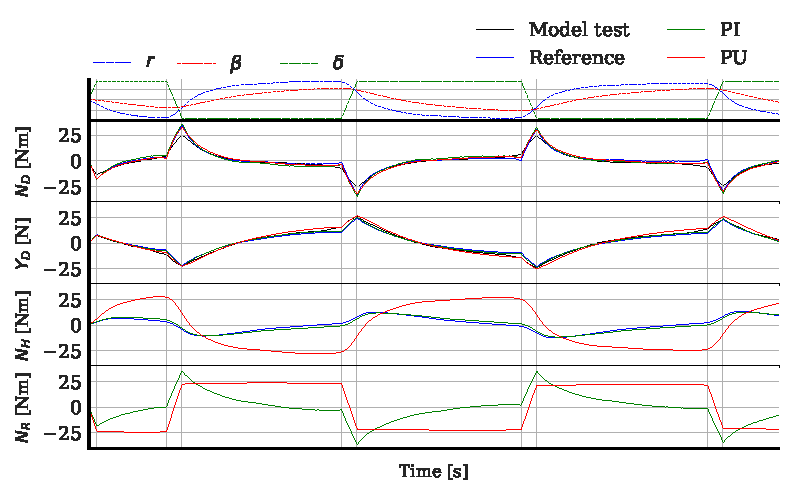
\includegraphics{kappa/images/results.ID_zigzag10.pdf}
    \caption{ID estimations of $Y_D$ and $N_D$ during a zigzag10/10 model test compared with model predictions.}
    \label{fig:ID_zigzag10}
\end{figure}
The hull forces can be further decomposed into contributions from the drift of the vessel, through the sway velocity $v$ and contributions from the yaw rate $r$, as shown in \autoref{fig:ID_regression_N_decomposition}. It seems that almost all the yawing moments $N_H$ depend on $r$ for the PU model and almost all the sway force $Y_H$ is generated by $v$, in contrast to the other two models where both $v$ and $r$ contribute to $N_H$ and $Y_H$.
\begin{figure}[h]
    \begin{center}
        \includesvg{kappa/images/results.hull_force_decomposition_zigzag20.svg}
        \caption{Decomposition of hull forces and moments during a zigzag20/20 test for parameters related to drift, yaw rate the prediction models.}
        \label{fig:ID_regression_N_decomposition}
    \end{center}
\end{figure}
So, the PU model not only has the wrong decomposition between rudder and hull forces, it also has the wrong decomposition of drift and yaw rate contributions within the hull force model. This is however not a big problem during the zigzag tests, where the drift and yaw rate are very correlated as seen from the phase plot in \autoref{fig:phase_portrait}. This can also explain why the completely data driven model from the previous paper (Paper \ref{pap:pit}) can get such good results, despite the erogenous decomposition.
\begin{figure}[h]
  \centering
  \includesvg{figures/multicollineraity.multicollinearity.svg}
  \caption{Phase portrait where the combination of drift angle and yaw rate is shown for zigzag10/10 and zigzag20/20 wPCC model tests.}
  \label{fig:phase_portrait}
\end{figure}
However, when the ship is exposed to wind so that the drift changes, an erroneous decomposition of the PU model is revealed, as shown in \autoref{fig:result_wind_state}. The PI model agrees better with the reference model in the wind state. Introducing a semi-empirical rudder model seems to have guided the identification toward a more physically correct model, with lower multicollinearity and better generalization from calm water zigzag tests to wind conditions.
\begin{figure}[h!]
    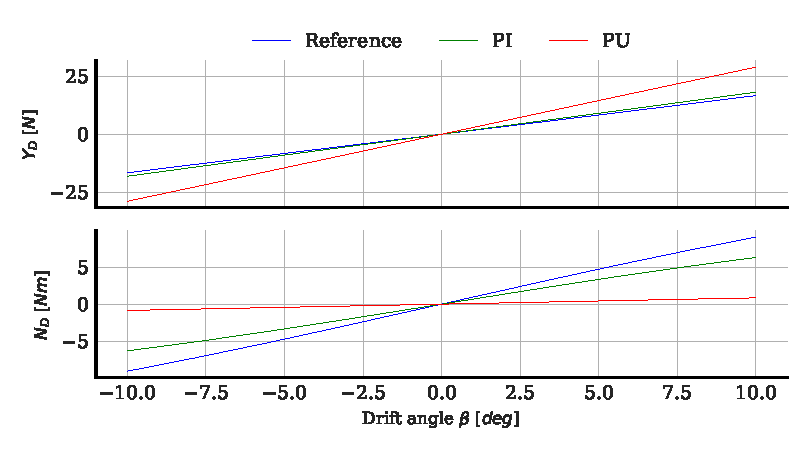
\includegraphics{kappa/images/result_wind_state.forces.pdf}
    \caption{Total sway force and yawing moment from the wPCC models at various drift angles.}
    \label{fig:result_wind_state}
\end{figure}

\FloatBarrier
%\subsection*{Comments}
\clearpage